\section{Integral de línea}

La integral de línea acumula una cantidad a lo largo de una curva $C$, que puede estar en el plano o en el espacio. En esta sección se estudia la integral de una función escalar respecto de la longitud de arco, denotada por
\[
\int_C f\,ds.
\]
La función $f$ asigna un valor a cada punto de la curva y $ds$ representa un elemento de longitud de la curva. Así como una integral doble suma contribuciones sobre pequeñas áreas y una integral triple sobre pequeños volúmenes, esta integral suma contribuciones sobre pequeños arcos.

Por ejemplo, si un alambre tiene densidad lineal variable, un tramo corto aporta aproximadamente su densidad multiplicada por su longitud. Al sumar esas masas se obtiene la masa del alambre. La misma idea permite calcular la carga de un hilo con densidad de carga conocida. Otro ejemplo es al tomar $f=1$, se obtiene la longitud de la curva. También permite definir el valor medio de una temperatura medida a lo largo de un cable.

Una parametrización describe los puntos de una curva mediante una función vectorial
\[
\vec r(t)=(x(t),y(t),z(t)),\qquad a\leq t\leq b.
\]
El parámetro $t$ identifica los puntos y su orden de recorrido. Una curva plana puede escribirse como $(x(t),y(t))$, o como $(x(t),y(t),0)$ si se considera dentro del espacio.

\begin{mydefinition}{Curva regular y curva regular por partes}
Una parametrización es regular si sus componentes tienen derivadas continuas y $\vec r\,'(t)\neq\vec 0$ en su intervalo. Se dice que es regular por partes si es continua y el intervalo puede dividirse en un número finito de subintervalos en los que la parametrización es regular, con derivadas laterales en los extremos. En los puntos de unión puede haber esquinas.
\end{mydefinition}

La continuidad por sí sola no garantiza regularidad. En lo que sigue se consideran curvas regulares por partes, recorridas una sola vez, salvo indicación contraria. En una curva cerrada se permite que coincidan los puntos inicial y final.

El vector $\vec r\,'(t)$ es tangente a la curva y su norma mide la rapidez de recorrido. La longitud acumulada desde $a$ y su diferencial son
\[
s(t)=\int_a^t\|\vec r\,'(u)\|\,du,
\qquad ds=\|\vec r\,'(t)\|\,dt,
\]
en cada tramo regular. En particular,
\[
L(C)=\int_a^b\sqrt{[x'(t)]^2+[y'(t)]^2+[z'(t)]^2}\,dt.
\]

Por ejemplo, la semicircunferencia superior de radio $2$ se parametriza mediante
\[
\vec r(t)=(2\cos t,2\sin t),\qquad 0\leq t\leq\pi.
\]
Sus extremos son $(2,0)$ y $(-2,0)$, y pasa por $(0,2)$ cuando $t=\pi/2$. Como $\|\vec r\,'(t)\|=2$, se tiene $ds=2\,dt$: un pequeño cambio angular $\Delta t$ corresponde a un arco de longitud $2\Delta t$.

\begingroup
\shorthandoff{>}
\begin{center}
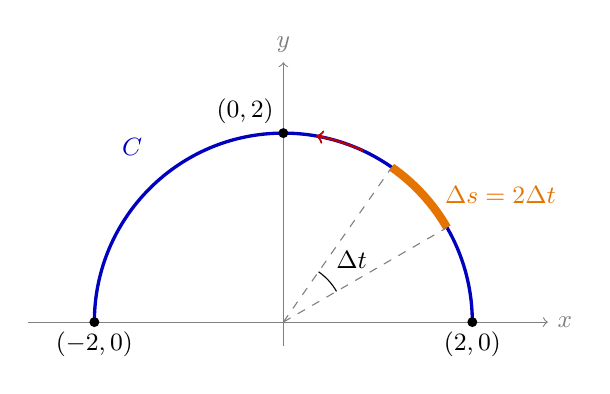
\begin{tikzpicture}[scale=1.2,every node/.style={font=\small}]
    \draw[->,gray] (-2.7,0) -- (2.8,0) node[right] {$x$};
    \draw[->,gray] (0,-.25) -- (0,2.75) node[above] {$y$};
    \draw[blue!75!black,very thick] (2,0) arc (0:180:2);
    \draw[orange!90!black,line width=3pt] (30:2) arc (30:55:2);
    \draw[->,red!75!black,thick] (65:2) arc (65:80:2);
    \draw[gray,dashed] (0,0) -- (30:2);
    \draw[gray,dashed] (0,0) -- (55:2);
    \draw (30:.65) arc (30:55:.65);
    \node at (42.5:.98) {$\Delta t$};
    \node[right,orange!90!black] at (40:2.1) {$\Delta s=2\Delta t$};
    \fill (2,0) circle (1.5pt) node[below] {$(2,0)$};
    \fill (-2,0) circle (1.5pt) node[below] {$(-2,0)$};
    \fill (0,2) circle (1.5pt) node[above left] {$(0,2)$};
    \node[blue!75!black] at (-1.6,1.85) {$C$};
\end{tikzpicture}
\end{center}
\endgroup

La figura distingue el incremento del parámetro, medido en radianes, de la longitud del arco naranja. El factor $\|\vec r\,'(t)\|$ realiza esa conversión también en curvas cuya rapidez no es constante.

\subsection{Construcción de la suma que define la integral}

Sea $f$ una función continua sobre una curva $C$. Se divide la curva, en orden de recorrido, mediante puntos $P_0,P_1,\ldots,P_n$. El arco $C_i$ comprendido entre $P_{i-1}$ y $P_i$ tiene longitud $\Delta s_i$. En cada arco se elige un punto de muestra
\[
P_i^*=(x_i^*,y_i^*,z_i^*).
\]
Cuando el arco es corto, $f$ varía poco sobre él, de modo que puede aproximarse por el valor constante $f(P_i^*)$. La contribución del arco es entonces aproximadamente $f(P_i^*)\Delta s_i$, y la contribución total se aproxima por
\[
S_{\mathcal P}=\sum_{i=1}^n f(P_i^*)\,\Delta s_i.
\]

\begingroup
\shorthandoff{>}
\begin{center}
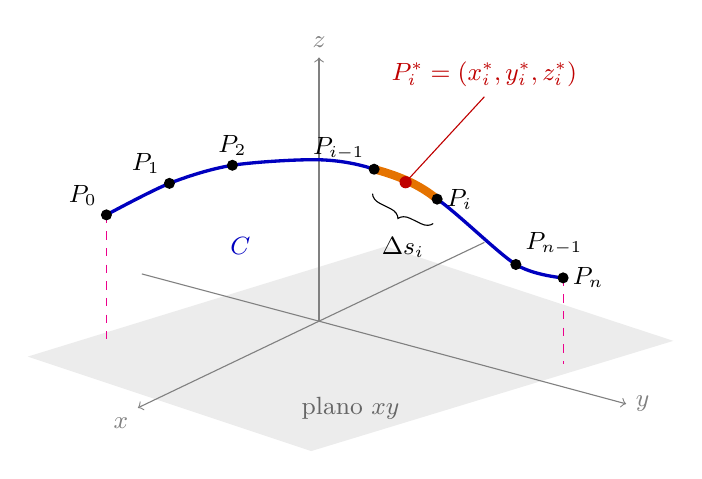
\begin{tikzpicture}[every node/.style={font=\small}]
    % Proyección esquemática de una curva espacial sobre el plano xy.
    \fill[gray!15] (-3.7,-.45) -- (-.1,-1.65) -- (4.5,-.25) -- (.85,.95) -- cycle;
    \draw[->,gray] (0,0) -- (-2.3,-1.1) node[below left] {$x$};
    \draw[->,gray] (0,0) -- (3.9,-1.05) node[right] {$y$};
    \draw[->,gray] (0,0) -- (0,3.35) node[above] {$z$};
    \draw[gray] (0,0) -- (2.1,1);
    \draw[gray] (0,0) -- (-2.25,.6);
    \draw[magenta,dashed] (-2.7,1.35) -- (-2.7,-.3);
    \draw[magenta,dashed] (3.1,.55) -- (3.1,-.55);
    \draw[blue!75!black,very thick] plot[smooth] coordinates
        {(-2.7,1.35) (-1.9,1.75) (-1.1,1.98) (0,2.05) (.7,1.93) (1.5,1.55) (2.5,.72) (3.1,.55)};
    \draw[orange!90!black,line width=3pt] (.7,1.93) .. controls (1,1.85) and (1.27,1.74) .. (1.5,1.55);
    \fill (-2.7,1.35) circle (2pt) node[above left] {$P_0$};
    \fill (-1.9,1.75) circle (2pt) node[above left] {$P_1$};
    \fill (-1.1,1.98) circle (2pt) node[above] {$P_2$};
    \fill (.7,1.93) circle (2pt) node[above left] {$P_{i-1}$};
    \fill (1.5,1.55) circle (2pt) node[right] {$P_i$};
    \fill (2.5,.72) circle (2pt) node[above right] {$P_{n-1}$};
    \fill (3.1,.55) circle (2pt) node[right] {$P_n$};
    \fill[red!75!black] (1.1,1.765) circle (2.2pt);
    \draw[red!75!black] (1.1,1.765) -- (2.1,2.85)
        node[above] {$P_i^*=(x_i^*,y_i^*,z_i^*)$};
    \draw[decorate,decoration={brace,mirror,amplitude=4pt}]
        (.68,1.62) -- (1.45,1.24) node[midway,below=7pt] {$\Delta s_i$};
    \node[blue!75!black] at (-1,.95) {$C$};
    \node[gray!80!black] at (.4,-1.1) {plano $xy$};
\end{tikzpicture}
\end{center}
\endgroup

El tramo naranja es un arco de la curva espacial, $\Delta s_i$ mide su longitud real, no la de su proyección sobre $xy$ ni la de la cuerda que une sus extremos. El punto rojo proporciona el valor de $f$ usado en ese tramo.

Si $f=\rho$ es una densidad lineal en $\mathrm{kg}/\mathrm{m}$ y $\Delta s_i$ se mide en metros, entonces
\[
\Delta m_i\approx\rho(P_i^*)\Delta s_i
\]
se mide en kilogramos. Esta interpretación explica por qué cada valor de la función se multiplica por una longitud antes de sumarlo.

\subsection{Definición de la integral de línea}

\begin{mydefinition}{Integral de línea respecto de la longitud de arco}
Sea $C$ una curva regular por partes y sea $f:C\to\mathbb R$ continua. Para una partición $\mathcal P$ de $C$ en arcos de longitudes $\Delta s_i$, se define
\[
\|\mathcal P\|=\max_{1\leq i\leq n}\Delta s_i.
\]
La integral de línea de $f$ sobre $C$ respecto de la longitud de arco es
\[
\int_C f\,ds
=\lim_{\|\mathcal P\|\to0}\sum_{i=1}^n f(P_i^*)\Delta s_i.
\]
Bajo estas hipótesis el límite existe y es independiente de los puntos de muestra y de las particiones elegidas. En el espacio se escribe $\int_C f(x,y,z)\,ds$ y en el plano, $\int_C f(x,y)\,ds$.
\end{mydefinition}

La condición $\|\mathcal P\|\to0$ exige que todos los arcos se hagan pequeños. Aumentar solamente el número de arcos no basta si alguno conserva una longitud fija.

Cuando $f=1$, cada sumando es $\Delta s_i$, por lo que
\[
\int_C1\,ds=L(C).
\]
Si $f\geq0$, la integral es no negativa. Si $f$ toma valores de ambos signos, las contribuciones pueden cancelarse. El diferencial $ds$ siempre representa longitud; el signo lo aporta $f$.

\subsection{Cómo evaluar una integral de línea}

\begin{mytheorem}{Evaluación mediante una parametrización}
Sea $\vec r:[a,b]\to\mathbb R^3$ una parametrización regular por partes que recorre $C$ una sola vez, y sea $f$ continua sobre $C$. Entonces
\[
\int_C f(x,y,z)\,ds
=\int_a^b f(x(t),y(t),z(t))\,
\sqrt{[x'(t)]^2+[y'(t)]^2+[z'(t)]^2}\,dt.
\]
Para una curva plana se omite la componente $z$. Si hay varios tramos regulares, se suman las integrales de esos tramos.
\end{mytheorem}

\begin{proof}
En un tramo regular, $s(t)=\int_a^t\|\vec r\,'(u)\|\,du$ es estrictamente creciente porque $\|\vec r\,'(t)\|>0$. Por ello tiene una inversa continua $t=t(s)$, con $0\leq s\leq L(C)$. La función $F(s)=f(\vec r(t(s)))$ es continua.

Una partición de $C$ en arcos corresponde a una partición de $[0,L(C)]$ con incrementos $\Delta s_i$. Las sumas de la definición son precisamente las sumas de Riemann de $F$. En consecuencia, el límite existe y
\[
\int_C f\,ds=\int_0^{L(C)}F(s)\,ds.
\]
El cambio de variable $s=s(t)$, con $s'(t)=\|\vec r\,'(t)\|$, da
\[
\int_0^{L(C)}F(s)\,ds
=\int_a^b f(\vec r(t))\|\vec r\,'(t)\|\,dt.
\]
Para una curva regular por partes se aplica el argumento a cada tramo. Las sumas se separan en esos tramos; los arcos que contienen puntos de unión tienen contribución que tiende a cero al refinar la partición, pues $f$ está acotada y hay un número finito de uniones. Así se obtiene la suma de las integrales correspondientes.
\end{proof}

Para el cálculo de $\int_C f\,ds$ se elige una parametrización y su intervalo, se sustituye la curva en $f$ y se calcula $ds=\|\vec r\,'(t)\|\,dt$. Después se evalúa la integral de una variable resultante. Los límites deben describir exactamente el arco indicado.

Si $C$ es la gráfica $y=g(x)$, con $g$ continuamente diferenciable en $[a,b]$, se puede usar $\vec r(t)=(t,g(t))$. La fórmula se convierte en
\[
\int_C f(x,y)\,ds
=\int_a^b f(x,g(x))\sqrt{1+[g'(x)]^2}\,dx.
\]

Cabe mencionar que $ds$ no es igual a $dt$ ni a $dx$. El factor de longitud no puede omitirse. Dos parametrizaciones regulares de la misma curva, recorrida una sola vez, producen el mismo valor de $\int_C f\,ds$, incluso si tienen sentidos opuestos. Si se recorre la curva dos veces, se cuentan dos veces sus contribuciones.

Para justificar la independencia del parámetro, si $t=\phi(u)$ es un cambio regular y monótono, la regla de la cadena da
\[
\left\|\frac{d}{du}\vec r(\phi(u))\right\|
=\|\vec r\,'(\phi(u))\|\,|\phi'(u)|.
\]
El cambio de variable en la integral compensa tanto la rapidez como el sentido de recorrido. El valor absoluto mantiene positiva la longitud cuando $\phi$ es decreciente.

También se conservan la linealidad y la aditividad: para funciones continuas $f,g$, constantes $\alpha,\beta$ y tramos consecutivos $C_1,C_2$ que solo comparten extremos,
\[
\int_C(\alpha f+\beta g)\,ds
=\alpha\int_C f\,ds+\beta\int_C g\,ds,
\qquad
\int_{C_1\cup C_2}f\,ds=\int_{C_1}f\,ds+\int_{C_2}f\,ds.
\]

\paragraph{Ejemplo 1. Una función sobre un arco de parábola}

Se desea evaluar $\int_C x\,ds$, donde $C$ es la porción de $y=x^2$ desde $(0,0)$ hasta $(1,1)$. La figura muestra la curva de integración y un arco corto; la integral acumula valores sobre la curva, no sobre el área situada debajo de ella.

\begingroup
\shorthandoff{>}
\begin{center}
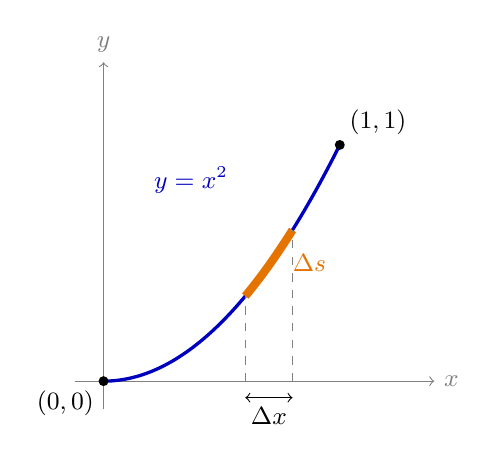
\begin{tikzpicture}[scale=3,every node/.style={font=\small}]
    \draw[->,gray] (-.12,0) -- (1.4,0) node[right] {$x$};
    \draw[->,gray] (0,-.12) -- (0,1.35) node[above] {$y$};
    \draw[blue!75!black,very thick,domain=0:1,samples=60] plot (\x,{\x*\x});
    \draw[orange!90!black,line width=3pt,domain=.6:.8,samples=15] plot (\x,{\x*\x});
    \draw[dashed,gray] (.6,0) -- (.6,.36);
    \draw[dashed,gray] (.8,0) -- (.8,.64);
    \draw[<->] (.6,-.07) -- (.8,-.07) node[midway,below] {$\Delta x$};
    \node[right,orange!90!black] at (.76,.5) {$\Delta s$};
    \fill (0,0) circle (.6pt) node[below left] {$(0,0)$};
    \fill (1,1) circle (.6pt) node[above right] {$(1,1)$};
    \node[blue!75!black] at (.37,.85) {$y=x^2$};
\end{tikzpicture}
\end{center}
\endgroup

Se toma $\vec r(t)=(t,t^2)$, $0\leq t\leq1$. Entonces
\[
f(\vec r(t))=t,\qquad
\vec r\,'(t)=(1,2t),\qquad ds=\sqrt{1+4t^2}\,dt.
\]
La sustitución $u=1+4t^2$, $du=8t\,dt$, permite evaluar
\begin{align*}
\int_C x\,ds
&=\int_0^1 t\sqrt{1+4t^2}\,dt
=\frac18\int_1^5 u^{1/2}\,du\\
&=\frac1{12}\left[u^{3/2}\right]_1^5
=\frac{5\sqrt5-1}{12}.
\end{align*}
En la figura, $\Delta s$ es mayor que su proyección horizontal $\Delta x$. El factor $\sqrt{1+4t^2}$ tiene en cuenta esa diferencia y aumenta donde la parábola se inclina más.

\paragraph{Ejemplo 2. Altura acumulada sobre una semicircunferencia}

Se considera $\int_C y\,ds$, donde $C$ es la semicircunferencia $x^2+y^2=4$, $y\geq0$. Como en la figura del recordatorio, se usa
\[
\vec r(t)=(2\cos t,2\sin t),\qquad 0\leq t\leq\pi.
\]
La norma de la derivada y la integral son
\begin{align*}
\|\vec r\,'(t)\|
&=\sqrt{4\sin^2t+4\cos^2t}=2,\\
\int_C y\,ds
&=\int_0^\pi (2\sin t)\,2\,dt
=4[-\cos t]_0^\pi=8.
\end{align*}

Esta integral admite una interpretación gráfica: sobre cada punto $(x,y)$ del arco se levanta una altura $z=f(x,y)=y$. Se obtiene una cortina vertical cuya base es $C$. Una tira corta tiene área aproximada $f(P_i^*)\Delta s_i$, por lo que el área de la cortina es $\int_C y\,ds$.

\begingroup
\shorthandoff{>}
\begin{center}
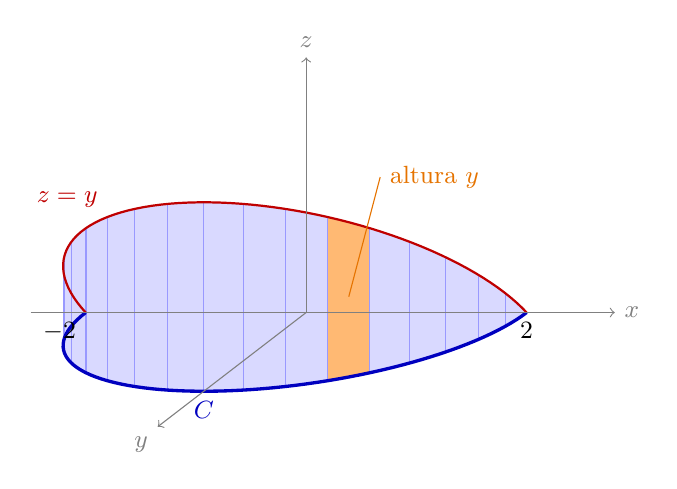
\begin{tikzpicture}[x={(1.4cm,0cm)},y={(-.65cm,-.5cm)},z={(0cm,1.2cm)},every node/.style={font=\small}]
    \foreach \ang in {0,10,...,170} {
        \fill[blue!15] ({2*cos(\ang)},{2*sin(\ang)},0)
            -- ({2*cos(\ang+10)},{2*sin(\ang+10)},0)
            -- ({2*cos(\ang+10)},{2*sin(\ang+10)},{2*sin(\ang+10)})
            -- ({2*cos(\ang)},{2*sin(\ang)},{2*sin(\ang)}) -- cycle;
    }
    \fill[orange!55] ({2*cos(50)},{2*sin(50)},0)
        -- ({2*cos(60)},{2*sin(60)},0)
        -- ({2*cos(60)},{2*sin(60)},{2*sin(60)})
        -- ({2*cos(50)},{2*sin(50)},{2*sin(50)}) -- cycle;
    \foreach \ang in {10,20,...,170} {
        \draw[blue!40] ({2*cos(\ang)},{2*sin(\ang)},0)
            -- ({2*cos(\ang)},{2*sin(\ang)},{2*sin(\ang)});
    }
    \draw[blue!75!black,very thick,domain=0:180,samples=70]
        plot ({2*cos(\x)},{2*sin(\x)},0);
    \draw[red!75!black,thick,domain=0:180,samples=70]
        plot ({2*cos(\x)},{2*sin(\x)},{2*sin(\x)});
    \draw[->,gray] (-2.5,0,0) -- (2.8,0,0) node[right] {$x$};
    \draw[->,gray] (0,0,0) -- (0,2.9,0) node[below left] {$y$};
    \draw[->,gray] (0,0,0) -- (0,0,2.7) node[above] {$z$};
    \node[below] at (2,0,0) {$2$};
    \node[below left] at (-2,0,0) {$-2$};
    \node[blue!75!black,below] at (0,2,0) {$C$};
    \draw[orange!90!black] (.3,-.8,1.1) node[right] {altura $y$}
        -- ({2*cos(55)},{2*sin(55)},.85);
    \node[red!75!black,above left] at (-1,1.732,1.732) {$z=y$};
\end{tikzpicture}
\end{center}
\endgroup

La cortina tiene altura cero en los extremos y altura $2$ en el punto medio del arco. La tira naranja aproxima una contribución a su área. Esta interpretación como área requiere una curva base plana y una función no negativa; en general, una integral de línea no representa un área.

\paragraph{Ejemplo 3. Una función sobre una hélice}

Se desea evaluar $\int_C z\,ds$ sobre una vuelta de la hélice
\[
\vec r(t)=(\cos t,\sin t,t),\qquad 0\leq t\leq2\pi.
\]
La curva rodea el cilindro $x^2+y^2=1$ mientras su altura crece desde $0$ hasta $2\pi$. Su proyección sobre $xy$ es la circunferencia unitaria.

\begingroup
\shorthandoff{>}
\begin{center}
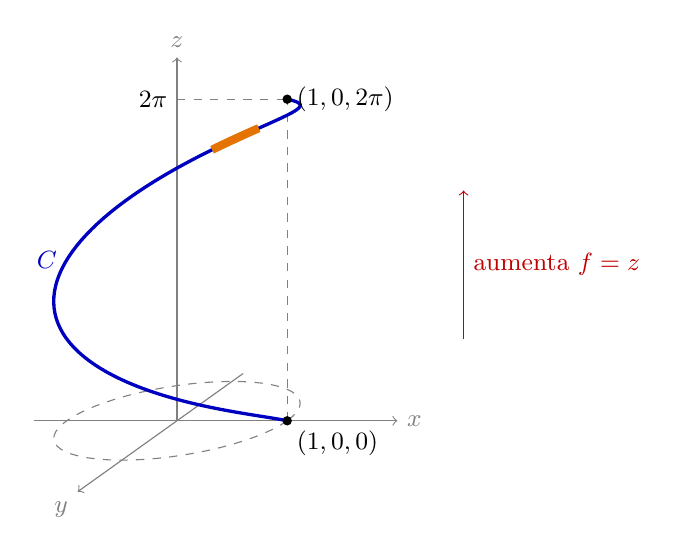
\begin{tikzpicture}[x={(1.4cm,0cm)},y={(-.7cm,-.5cm)},z={(0cm,.65cm)},every node/.style={font=\small}]
    \draw[gray,dashed,domain=0:360,samples=60] plot ({cos(\x)},{sin(\x)},0);
    \draw[gray,dashed] (1,0,0) -- (1,0,{2*pi});
    \draw[gray,dashed] (0,0,{2*pi}) -- (1,0,{2*pi});
    \draw[->,gray] (-1.3,0,0) -- (2,0,0) node[right] {$x$};
    \draw[->,gray] (0,-1.2,0) -- (0,1.8,0) node[below left] {$y$};
    \draw[->,gray] (0,0,0) -- (0,0,7.1) node[above] {$z$};
    \draw[blue!75!black,very thick,domain=0:360,samples=100]
        plot ({cos(\x)},{sin(\x)},{\x*pi/180});
    \draw[orange!90!black,line width=3pt,domain=260:285,samples=15]
        plot ({cos(\x)},{sin(\x)},{\x*pi/180});
    \fill (1,0,0) circle (1.7pt) node[below right] {$(1,0,0)$};
    \fill (1,0,{2*pi}) circle (1.7pt) node[right] {$(1,0,2\pi)$};
    \node[left] at (0,0,{2*pi}) {$2\pi$};
    \node[blue!75!black,left] at (-1,0,3.14) {$C$};
    \draw[->,red!75!black] (2.6,0,1.6) -- (2.6,0,4.5)
        node[midway,right] {aumenta $f=z$};
\end{tikzpicture}
\end{center}
\endgroup

Se tiene
\[
\vec r\,'(t)=(-\sin t,\cos t,1),\qquad
\|\vec r\,'(t)\|=\sqrt{\sin^2t+\cos^2t+1}=\sqrt2.
\]
Por tanto,
\[
\int_C z\,ds
=\int_0^{2\pi} t\sqrt2\,dt
=\sqrt2\left[\frac{t^2}{2}\right]_0^{2\pi}
=2\sqrt2\,\pi^2.
\]
Los arcos de igual longitud aportan más cerca del extremo superior porque allí $z$ es mayor. La proyección circular, por sí sola, perdería tanto la altura del integrando como la componente vertical de la longitud.

\subsection{Aplicaciones}

Un alambre delgado se modela mediante una curva $C$ y una densidad lineal continua $\rho:C\to[0,\infty)$. La densidad indica masa por unidad de longitud. Su masa total es
\[
m=\int_C\rho\,ds.
\]
Si la densidad es constante, $\rho=\rho_0$, se obtiene $m=\rho_0L(C)$. Cuando varía, cada arco debe ponderarse por su densidad local.

\paragraph{Ejemplo. Alambre semicircular más denso en la parte superior}

Un alambre ocupa la semicircunferencia $x^2+y^2=4$, $y\geq0$, con coordenadas medidas en metros. Su densidad es
\[
\rho(x,y)=\rho_0\left(1+\frac{y}{\ell}\right),
\qquad \rho_0=1\,\mathrm{kg}/\mathrm{m},\qquad \ell=1\,\mathrm{m}.
\]
La razón $y/\ell$ es adimensional. La densidad vale $1\,\mathrm{kg}/\mathrm{m}$ en los extremos y $3\,\mathrm{kg}/\mathrm{m}$ en el punto más alto.

\begingroup
\shorthandoff{>}
\begin{center}
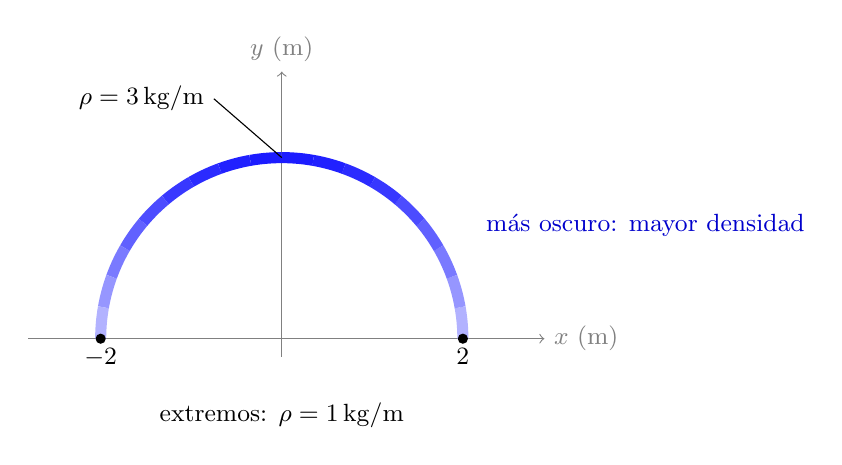
\begin{tikzpicture}[scale=1.15,every node/.style={font=\small}]
    \draw[->,gray] (-2.8,0) -- (2.9,0) node[right] {$x\ (\mathrm m)$};
    \draw[->,gray] (0,-.2) -- (0,2.95) node[above] {$y\ (\mathrm m)$};
    \foreach \ang in {0,10,...,170} {
        \pgfmathtruncatemacro{\tono}{25+65*sin(\ang+5)}
        \draw[blue!\tono!white,line width=4pt,domain=\ang:({\ang+10}),samples=8]
            plot ({2*cos(\x)},{2*sin(\x)});
    }
    \fill (2,0) circle (1.6pt) node[below] {$2$};
    \fill (-2,0) circle (1.6pt) node[below] {$-2$};
    \draw (0,2) -- (-.75,2.65) node[left] {$\rho=3\,\mathrm{kg}/\mathrm m$};
    \node[below] at (0,-.6) {extremos: $\rho=1\,\mathrm{kg}/\mathrm m$};
    \node[right,blue!80!black] at (2.15,1.25) {más oscuro: mayor densidad};
\end{tikzpicture}
\end{center}
\endgroup

Se usa $\vec r(t)=(2\cos t,2\sin t)$ en metros, con $0\leq t\leq\pi$. Entonces $ds=2\,dt$ en metros y $\rho(\vec r(t))=1+2\sin t$ en $\mathrm{kg}/\mathrm m$. Sustituyendo estos valores numéricos en las unidades indicadas,
\begin{align*}
m&=\left(\int_0^\pi(1+2\sin t)\,2\,dt\right)\mathrm{kg}\\
&=\left(2\pi+4[-\cos t]_0^\pi\right)\mathrm{kg}
=(2\pi+8)\,\mathrm{kg}.
\end{align*}
El término $2\pi\,\mathrm{kg}$ es la masa que tendría el alambre con densidad uniforme $\rho_0$; los $8\,\mathrm{kg}$ adicionales proceden del incremento de densidad con la altura. Como su longitud es $2\pi\,\mathrm m$ y su densidad está entre $1$ y $3\,\mathrm{kg}/\mathrm m$, la masa debe estar entre $2\pi$ y $6\pi\,\mathrm{kg}$, lo cual concuerda con el resultado.

\subsection{Ejercicios}

\begin{enumerate}
    \begin{samepage}
    \item Grafique las curvas siguientes, indique sus extremos y determine el elemento de longitud $ds$ en cada caso:
\begin{enumerate}
    \item $\vec r(t)=(3t,4t)$, $0\leq t\leq1$.
    \item $\vec r(t)=(2\cos t,2\sin t)$, $0\leq t\leq\pi/2$.
    \item $\vec r(t)=(\cos t,\sin t,2t)$, $0\leq t\leq2\pi$.
\end{enumerate}

    \end{samepage}
    \item Un alambre se divide en cuatro arcos de longitudes $0.2$, $0.3$, $0.1$ y $0.4\,\mathrm m$. Las densidades lineales medidas en un punto de cada arco son, respectivamente, $2$, $3$, $4$ y $2\,\mathrm{kg}/\mathrm m$. Formule la suma que aproxima su masa y evalúela. Explique qué condición deben cumplir las longitudes de los arcos al refinar la partición para obtener la integral de línea.

    \item Evalúe $\int_C1\,ds$, donde $C$ es el segmento de $(0,0,0)$ a $(2,3,6)$. Interprete el resultado y compruébelo mediante la distancia entre los extremos.

    \item Evalúe $\int_C(x+y)\,ds$, donde $C$ es el segmento que une $(0,0)$ con $(2,2)$.

    \item Evalúe $\int_C x^2\,ds$, donde $C$ es el cuarto de circunferencia $x^2+y^2=9$ situado en el primer cuadrante. Grafique el arco de integración.

    \item Evalúe $\int_C y\,ds$, donde $C$ es el arco de la parábola $x=y^2$ desde $(0,0)$ hasta $(4,2)$.

    \item Evalúe $\int_C(x^2+y^2+z)\,ds$, donde
\[
\vec r(t)=(2\cos t,2\sin t,3t),\qquad 0\leq t\leq2\pi.
\]
Describa la curva y su proyección sobre el plano $xy$.

    \item Calcule el área de la cortina vertical cuya base es el cuarto de circunferencia $x^2+y^2=4$ en el primer cuadrante y cuya altura es $f(x,y)=x+y$. Represente la base y las alturas en sus extremos.

    \item Evalúe $\int_C y\,ds$ para cada una de las siguientes curvas que unen $(0,0)$ con $(1,1)$ y compare los resultados:
\begin{enumerate}
    \item El segmento de recta entre ambos puntos.
    \item La trayectoria formada por el segmento de $(0,0)$ a $(1,0)$ seguido del segmento de $(1,0)$ a $(1,1)$.
\end{enumerate}
Explique si la integral queda determinada únicamente por los extremos de la curva.

    \item Un alambre ocupa el cuarto de circunferencia $x^2+y^2=R^2$ en el primer cuadrante, donde $R>0$ es una longitud. Su densidad lineal es
\[
\rho(x,y)=\rho_0\left(1+\frac{x}{R}\right),\qquad \rho_0>0,
\]
con $\rho_0$ en unidades de masa por longitud. Calcule su masa y su densidad media $\rho_{\mathrm{med}}=m/L(C)$. Indique en qué extremo es mayor la densidad.

    \item Un alambre tiene la forma de la hélice
\[
\vec r(t)=(a\cos t,a\sin t,bt),\qquad 0\leq t\leq2\pi,
\]
donde $a,b>0$ son longitudes. Su densidad es $\rho(x,y,z)=\rho_0(1+z/b)$, con $\rho_0>0$ en unidades de masa por longitud. Determine su masa y compárela con la de un alambre de la misma forma y densidad constante $\rho_0$.

    \item Evalúe $\int_C y\,ds$ sobre la semicircunferencia superior unitaria usando cada una de las parametrizaciones
\[
\vec r_1(t)=(\cos t,\sin t),\quad 0\leq t\leq\pi,
\qquad
\vec r_2(u)=(-\cos(2u),\sin(2u)),\quad 0\leq u\leq\pi/2.
\]
Compare las rapideces, los sentidos de recorrido y los valores de las integrales. Explique por qué las integrales $\int_0^\pi\sin t\,dt$ y $\int_0^{\pi/2}\sin(2u)\,du$, sin el factor de longitud correspondiente, no producen el mismo resultado.

    \item Sea $C$ una curva regular por partes de longitud $L>0$ y sea $f:C\to\mathbb R$ continua, con $A\leq f(P)\leq B$ para todo $P\in C$. Demuestre que
\[
AL\leq\int_C f\,ds\leq BL.
\]
Deduzca que el valor medio $f_{\mathrm{med}}=\frac1L\int_C f\,ds$ está entre $A$ y $B$.

    \item Sea $C$ una curva parametrizada por una función regular $\vec r:[a,b]\to\mathbb R^3$ que la recorre una sola vez, y sea $f$ continua sobre $C$. Demuestre directamente, mediante $\widetilde{\vec r}(u)=\vec r(a+b-u)$ para $a\leq u\leq b$, que invertir el sentido de recorrido conserva el valor de $\int_C f\,ds$.

    \item Sea $C$ una curva regular por partes y sea $\lambda>0$. La curva $C_\lambda$ se obtiene multiplicando por $\lambda$ todas las coordenadas de los puntos de $C$. Sea $f$ continua en $\mathbb R^3$ y suponga que existe un número real $k$ tal que
\[
f(\lambda x,\lambda y,\lambda z)=\lambda^k f(x,y,z)
\]
para todo $(x,y,z)\in\mathbb R^3$ y todo $\lambda>0$. Demuestre que
\[
\int_{C_\lambda} f\,ds=\lambda^{k+1}\int_C f\,ds.
\]
Interprete el caso $f=1$ y determine cómo cambia $\int_C(x^2+y^2+z^2)\,ds$ cuando se duplican todas las coordenadas de la curva.

\end{enumerate}
